% Use only LaTeX2e, calling the article.cls class and 12-point type.

\documentclass[12pt]{article}

% Users of the {thebibliography} environment or BibTeX should use the
% scicite.sty package, downloadable from *Science* at
% http://www.sciencemag.org/authors/preparing-manuscripts-using-latex 
% This package should properly format in-text
% reference calls and reference-list numbers.

\usepackage{scicite}

\usepackage{times}

% The preamble here sets up a lot of new/revised commands and
% environments.  It's annoying, but please do *not* try to strip these
% out into a separate .sty file (which could lead to the loss of some
% information when we convert the file to other formats).  Instead, keep
% them in the preamble of your main LaTeX source file.

\usepackage{verbatim}
\usepackage{amsmath}
\usepackage{dsfont}
\usepackage{amssymb}
\usepackage{tipa}
\usepackage{graphicx}
\usepackage{booktabs}
% The following parameters seem to provide a reasonable page setup.

\topmargin 0.0cm
\oddsidemargin 0.2cm
\textwidth 16cm 
\textheight 21cm
\footskip 1.0cm

\newcommand{\indicator}{\mathds{1}} %{{\rm I\kern-.3em E}}

\usepackage{phonrule}

%The next command sets up an environment for the abstract to your paper.

\newenvironment{sciabstract}{%
\begin{quote} \bf}
{\end{quote}}



% Include your paper's title here

\title{Synthesizing Theories of Human Language with Bayesian Program Induction} 


% Place the author information here.  Please hand-code the contact
% information and notecalls; do *not* use \footnote commands.  Let the
% author contact information appear immediately below the author names
% as shown.  We would also prefer that you don't change the type-size
% settings shown here.

%% \author
%% {John Smith,$^{1\ast}$ Jane Doe,$^{1}$ Joe Scientist$^{2}$\\
%% \\
%% \normalsize{$^{1}$Department of Chemistry, University of Wherever,}\\
%% \normalsize{An Unknown Address, Wherever, ST 00000, USA}\\
%% \normalsize{$^{2}$Another Unknown Address, Palookaville, ST 99999, USA}\\
%% \\
%% \normalsize{$^\ast$To whom correspondence should be addressed; E-mail:  jsmith@wherever.edu.}
%% }

% Include the date command, but leave its argument blank.

\date{}



%%%%%%%%%%%%%%%%% END OF PREAMBLE %%%%%%%%%%%%%%%%



\begin{document} 

% Double-space the manuscript.

\baselineskip24pt

% Make the title.

\maketitle 



% Place your abstract within the special {sciabstract} environment.

\begin{sciabstract}
\end{sciabstract}



% In setting up this template for *Science* papers, we've used both
% the \section* command and the \paragraph* command for topical
% divisions.  Which you use will of course depend on the type of paper
% you're writing.  Review Articles tend to have displayed headings, for
% which \section* is more appropriate; Research Articles, when they have
% formal topical divisions at all, tend to signal them with bold text
% that runs into the paragraph, for which \paragraph* is the right
% choice.  Either way, use the asterisk (*) modifier, as shown, to
% suppress numbering.

\section*{Introduction}

An age-old aspiration within artificial intelligence research is to
build a machine that helps automate the scientific process by
synthesizing theories or
models~\cite{paul1990autonomous,langley1987scientific,schmidt2009distilling}.
This aspiration remains largely unrealized: despite small-scale
demonstrations of machine-assisted theory
induction~\cite{Langley1981BACON5TD,schmidt2009distilling}, practicing
scientists do not use machines to generate theories.  In contrast, AI
has made great strides on problems like machine vision and natural
language processing.  How can the artificial intelligence community
get theory induction off the ground?  This is an especially difficult
question, because the current mainstream in machine intelligence
focuses on qualitatively different classes of problems (e.g.,
prediction tasks like classification and regression), whereas theory
induction requires synthesizing human-understandable causal models of
real-world phenomena~\cite{pearl2009causality}, so that human
scientists can understand and learn from the AI's outputs.

Theory induction is a challenge both for the natural sciences and AI,
with connections to questions in cognitive development.
Children, like scientists,
build systems of laws and concepts
to explain the world around them,
building intuitive theories of kinship, biology, physics, number,
grammar, and other domains, motivating the `child as scientist' metaphor~\cite{childAsScientist}.
To bridge these different kinds of theory induction---in scientists, children, and machines---
we propose theory induction research start with theories of human language,
for several reasons.
First, scientists, specifically linguists,
%% build theories of language starting from
%% experimental data (utterances paired with their meanings),
%% and 
have compiled large corpora 
from a variety of languages,
giving a rich and varied dataset for benchmarking theory induction algorithms.
Second, children easily acquire language from
modest amounts of data,
suggesting that
inducing theories of language is tractable,
even from sparse data;
and also suggesting that accounts of
linguistic theory induction
could shed light on language acquisition.
Going back to at least Chomsky,
linguists have sometimes thought of the acquisition problem as
approximating the problem facing the linguist~\cite{chomsky1956three,chomsky1988current}.
Third,
theories of language
are traditionally formalized in computational terms,
exposing a suite of formalisms ready to be deployed by AI researchers.
These three features of human language --- the availability of many highly-varied datasets,
the interfaces with cognitive development,
and the computational formalisms within linguistics ---
conspire to single out language as an especially suitable target for
research in automated theory induction.



We have proposed theory induction research start with theories of human
language, and here introduce a model of theory induction for a
key module of natural language: \emph{morphophonology}, the
relationship between word pronunciation and meaning.
Acquiring the morphophonology of a language involve solving a basic
problem confronting both linguists and children: given a collection
of utterances, together with aspects of their meaning, what is the
causal relationship between form and meaning?
\begin{comment}
Morphophonology, and
natural language more broadly, presents a tractable challenge to
theory induction, for three reasons.  First, every natural language is
a different theory induction problem, so there is a wide spectrum of
induction tasks to evaluate on.  Second, linguistics as a field
traditionally formalizes theories in computational terms, and so there
is a pre-existing body of representations and algorithms for the AI
researcher to draw upon.  Third, we know that acquiring theories of
language (e.g., grammars) is tractable, because children 
acquire language, and field linguists can be trained to build theories of grammar.
\end{comment}
Our contribution is a model for synthesizing theories of natural
language morphophonology.  Like linguists, the model starts with a
collection of utterances paired with meanings, and then constructs a
causal, interpretable model explaining how those meanings gave rise to
the utterances, roughly mirroring the process by which theorists
construct theories starting from experimental data.  In addition to
building theories, scientists distill those theories into higher-level
kinds of knowledge spanning multiple theories (e.g., energy
conservation and Lorentz invariance in physics; XXX in chemistry;
universal grammar in linguistics).  We argue that this higher-level
abstract knowledge is a crucial part of theory induction, imparting
prior knowledge and constraints on what would otherwise be an
ill-posed inductive reasoning problem.  Our model also acquires this
higher-level knowledge by jointly inferring theories for multiple
languages, and then shifting its inductive bias over theories to more
closely match the attested distribution of languages.  We evaluate our
algorithm on \# data sets spanning \# languages, automatically finding
theories that can model a wide swath of a core component of human
language.






\begin{figure}
  \includegraphics[width = \textwidth]{naturalLanguageGenerativeModel-crop.pdf}
  \caption{Agent induces theories (teal) for a range of languages, given observed form/meaning pairs (orange). Grammars are expressed as programs drawn from a universal grammar, or programming language (magenta). }\label{generativeModel}
  \end{figure}







\section*{Discovering Theories by Synthesizing Programs} 

We frame our approach as Bayesian Program Learning (BPL:
see~\cite{lake2015human}), where the model explains a set of
utterance/meaning pairs $\left\{(u_n,m_n) \right\}_{n = 1}^N$ by
inferring a theory $T$, which we model as a program.  Formalizing
grammars (theories) as generative programs has a long history in
linguistics~\cite{chomsky1968sound},
for two intuitive reasons: being procedural,
programs can capture the causal nature of
both grammars and theories;
and being highly structured,
programs can be interpreted by human scientists.
Written as a probabilistic
inference problem, our model seeks the theory $T$ maximizing
$P(\{u_n,m_n\}_{n = 1}^N | T)P(T|UG)$, where $UG$ is a ``universal
grammar'' encapsulating  higher-level abstract knowledge across
different languages.  In this BPL setting we model $UG$ as a prior
distribution over theories (programs), and represent programs as
Context-Sensitive Rewrites, a Turing-complete program representation,
but restrict the rewrites in such a way as to make them equivalent to
finite state transducers --- this approach comes from the computational
linguistics literature~\cite{beesley2003finite}.

A language's morphophonology can generate infinitely many
utterances,
depending on what words are in the language,
just as theories in other sciences
can generate an infinite set of
possible observations --- in Newtonian mechanics,
the theory prescribes
how bodies will interact,
but does not prescribe
the number of bodies or their masses.
Thus, for a theory to explain a set of observations,
it must introduce additional latent (unobserved)
variables on a dataset-by-dataset basis.
For the theories of language considered here,
this latent variable is the \emph{lexicon},
which is a mapping between
the meaning of a stem and its pronunciation.
Taking into account the latent lexicon,
we refine the theory-induction objective into
finding the theory $T$ and lexicon $L$ maximizing
$\left[\prod_{n = 1}^N \indicator[T\text{ and }L\text{ predict }u_n\text{ for }m_n] \right]P(L)P(T|UG)$.
Fig.~\ref{generativeModel} illustrates this set up for three different languages.

Although this framing captures the problem a BPL theory inductor needs to solve,
it offers no guidance on how to solve that problem:
the space of all programs (theories) is infinitely large and
sharply discontinuous, lacking the local smoothness that
enables local optimization algorithms (e.g., gradient descent; MCMC)
to succeed.
We adopt a strategy based on constraint--based program synthesis,
where the optimization problem is translated
into a combinatorial constraint satisfaction 
problem and solved using
a SMT solver~\cite{solar2006combinatorial}.
To scale these solvers to
large and complex theories 
we wrap the solver in
an outer loop that incrementally
introduces new (utterance, meaning) pairs,
incrementally modifying the theory to explain
new data points (Supplementary materials).

We apply our model to textbook morphophonology problems taken from~\cite{9780511808869}.
Each textbook problem requires synthesizing a
causal theory of a subset of a language.
Fig.~\ref{languageComparison}
compares model outputs against 
ground-truth textbook solutions.
These problem span a range of difficulties
and cover a diverse set of natural language phenomena:
systems for assigning tone (e.g., in Kerewe,
`to count' is kubala, but `to count it' is \textipa{kuk\'ib\'ala}, where accents mark high tones),
for ``harmonizing'' vowels (found across many languages, e.g. Kikuria
has s\underline{ii}ka meaning `close' but s\underline{ee}kera meaning `close for';
Latin has [ad\underline{e}ps] meaning `fat' (nominative)' but [ad\underline{i}pis] for the genitive `fat'),
and many other linguistic phenomena like
assimilation, epenthesis, and degemination (Fig.~\ref{exampleGrammars} and Supplementary materials).

Our theory induction model covers a wider range of languages and
phenomena than prior grammar induction algorithms from the
computational linguistics literature: prior approaches either recover
interpretable causal models
(e.g.,~\cite{Albright03rulesvs,gildea1996learning,rasin2015learning})
but do not scale to a wide range of challenging and realistic data
sets, or abandon theory induction and instead learn opaque
probabilistic models~\cite{cotterell-peng-eisner-2015} that may
nonetheless predict the data well but which do not help human
scientists generate theories.  Our improvement here stems from two
modeling choices: First, we use a generic computational substrate ---
context-sensitive rewrites --- giving the expressive power needed to
explain diverse linguist phenomena.  Second, we leverage solver-based
program synthesis techniques, borrowing decades of
research in the programming languages community that have honed these
tools to the point that we can scale them to
realistic data sets using rich program representations.

%2


\begin{figure}
  \begin{tabular}{lcc}    
    \toprule
    &  Tibetan Count System&Catalan Nouns\\\midrule
    \rotatebox[origin=c]{90}{Subset of Data}&
    
\begin{tabular}{ll}
1&\textipa{\|x{j}ig}\\
4&\textipa{\|x{s}i}\\
5&\textipa{Na}\\
9&\textipa{gu}\\
10&\textipa{\|x{j}u}\\
11 ($= 10 + 1$) & \textipa{\|x{j}ug\|x{j}ig}\\
14 ($= 10 + 4$) & \textipa{\|x{j}ub\|x{s}i}\\
15 ($= 10 + 5$) & \textipa{\|x{j}uNa}\\
19 ($= 10 + 9$) & \textipa{\|x{j}urgu}\\
40 ($= 4 + 10$) & \textipa{\|x{s}ib\|x{j}u}\\
50 ($= 5 + 10$) & \textipa{Nab\|x{j}u}\\
90 ($= 9 + 10$) & \textipa{gub\|x{j}u}
\end{tabular}
&
\begin{tabular}{lllll}
  \textipa{@kelj}$\sim$\textipa{@kelj@} &&\textipa{mal}$\sim$\textipa{mal@} \\
\textipa{siBil}$\sim$\textipa{siBil@} &&\textipa{@skerp}$\sim$\textipa{@skerp@} \\
\textipa{Sop}$\sim$\textipa{Sop@} &&\textipa{sEk}$\sim$\textipa{sEk@} \\
\textipa{@spEs}$\sim$\textipa{@spEs@} &&\textipa{gros}$\sim$\textipa{gros@} \\
\textipa{baS}$\sim$\textipa{baS@} &&\textipa{koS}$\sim$\textipa{koS@} \\
\textipa{tot}$\sim$\textipa{tot@} &&\textipa{brut}$\sim$\textipa{brut@} \\
\textipa{pOk}$\sim$\textipa{pOk@} &&\textipa{pr@sis}$\sim$\textipa{pr@siz@} \\
\textipa{fr@nses}$\sim$\textipa{fr@nsez@} &&\textipa{gris}$\sim$\textipa{griz@} \\
\textipa{k@zat}$\sim$\textipa{k@zaD@} &&\textipa{bwit}$\sim$\textipa{bwiD@} \\
\textipa{rOt\super S}$\sim$\textipa{rOZ@} &&\textipa{bot\super S}$\sim$\textipa{boZ@} \\
\textipa{orp}$\sim$\textipa{orB@} &&\textipa{ljark}$\sim$\textipa{ljarG@} \\
\textipa{sek}$\sim$\textipa{seG@} &&\textipa{f@Suk}$\sim$\textipa{f@SuG@} \\
\textipa{grok}$\sim$\textipa{groG@} &&\textipa{puruk}$\sim$\textipa{puruG@} \\
\textipa{kandit}$\sim$\textipa{kandiD@} &&\textipa{frEt}$\sim$\textipa{frED@} \\
\textipa{s@Gu}$\sim$\textipa{s@Gur@} &&\textipa{du}$\sim$\textipa{dur@} \\
\textipa{s@G@Do}$\sim$\textipa{s@G@Dor@} &&\textipa{kla}$\sim$\textipa{klar@} \\
\textipa{nu}$\sim$\textipa{nu@} &&\textipa{kru}$\sim$\textipa{kru@} \\
\textipa{flO\~nd\super Zu}$\sim$\textipa{flO\~nd\super Z@} &&\textipa{dropu}$\sim$\textipa{drop@} \\
\textipa{@gzakt@}$\sim$\textipa{@gzakt@} &&\textipa{@lBi}$\sim$\textipa{@lBin@} \\
\textipa{sa}$\sim$\textipa{san@} &&\textipa{pla}$\sim$\textipa{plan@} \\
\textipa{bo}$\sim$\textipa{bon@} &&\textipa{s@rE}$\sim$\textipa{s@rEn@} \\
\textipa{suBlim}$\sim$\textipa{suBlim@} &&\textipa{al}$\sim$\textipa{alt@} \\
\textipa{fOr}$\sim$\textipa{fOrt@} &&\textipa{kur}$\sim$\textipa{kurt@} \\
\textipa{sor}$\sim$\textipa{sorD@} &&\textipa{bEr}$\sim$\textipa{bErD@} \\
\textipa{san}$\sim$\textipa{sant@} &&\textipa{k@lEn}$\sim$\textipa{k@lEnt@} \\
\textipa{prufun}$\sim$\textipa{prufund@} &&\textipa{f@kun}$\sim$\textipa{f@kund@} \\
\textipa{d@sen}$\sim$\textipa{d@sent@} &&\textipa{dulen}$\sim$\textipa{dulent@} \\
\textipa{@stuDian}$\sim$\textipa{@stuDiant@} &&\textipa{blaN}$\sim$\textipa{blaNk@} & 
  \end{tabular}
\\\midrule 
\rotatebox[origin=c]{90}{Theory}&
\begin{tabular}{l}
  \phonb{C}{$\varnothing$}{\#}{C}\\
  (\emph{Upon encountering a consonant (C),}\\
  \emph{ delete it ($\to\varnothing$) at the beginning of}\\
  \emph{ a word (\#\_) if followed by another}\\
  \emph{ consonant (\_C)})
  \end{tabular}
&
\begin{tabular}{l}
Morphology:   stem$\sim$stem$+$\textipa{@}\\
  \phonr{[ +coronal +sonorant -lateral ]}{$\varnothing$}{\#}
\\\phonr{[ -sonorant ]}{[ -voice ]}{\#}
\\\phonl{C}{\textipa{k}}{\textipa{N}}
\\\phonb{[ +voice -nasal ]}{[ +continuant ]}{[ -nasal ]}{V}
\\\phonb{V}{$\varnothing$}{[ -sonorant ]}{V}
\\\phonb{\textipa{t}}{$\varnothing$}{C}{\#}
\end{tabular}
  \\
  \bottomrule  \end{tabular}
\caption{Example morphophonologies}
\label{exampleGrammars}
    \end{figure}


\begin{figure}
\centering\vspace{-3cm}  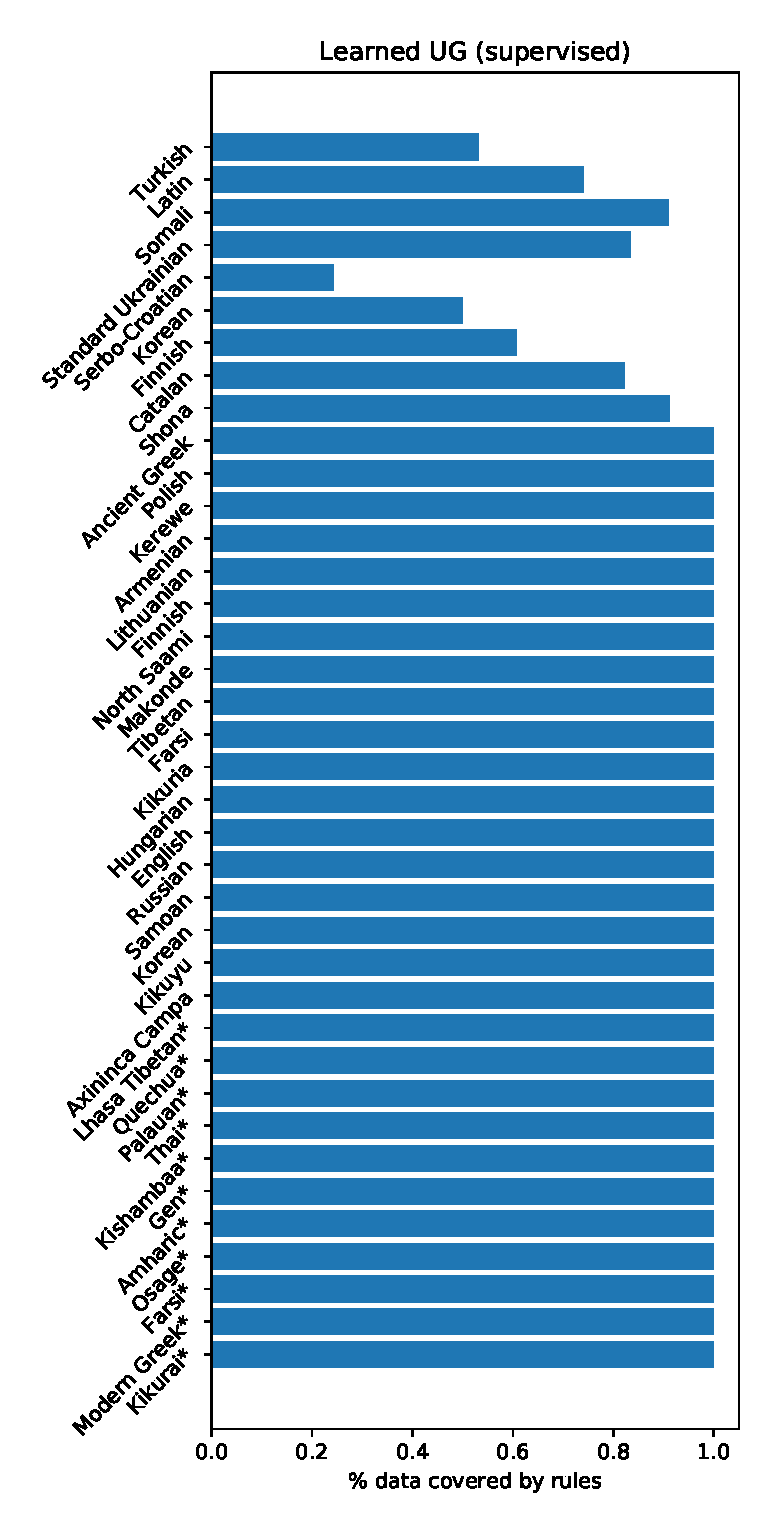
\includegraphics[width = 0.7\textwidth]{figures/languageComparison.eps}
  \caption{Program-synthesis-based phonological rule learner applied to 38 problems from a standard phonology textbook~\cite{9780511808869}. \% data covered by rules: fraction of the phonology problem that is explained by the learned program (so 100\% does not mean a \emph{perfect} solution, but a \emph{consistent} solution). Problems marked with an asterisk are very easy problems; the other problems are more challenging. Not shown: last eleven problems in the textbook, which are very hard: those results are pending.}\label{languageComparison}
\end{figure}

\section*{The Role of Higher-Level Knowledge}

No theory is built from scratch: instead, researchers borrow concepts
and constraints from other successful theories.  Linguistics has long
acknowledged the importance of constraints and inductive biases in
language learning, and these principles collectively go by the name
Universal Grammar: innate for child language learners and 
empirically probed by linguists.
In practice,
both children and linguists
may have very little data to go off,
and thus success often hinges upon
having the right kind of high-level knowledge.

Our model represents and acquires this cross-theory knowledge
by jointly inferring $UG$ along with the grammars for each data set.
Assuming we have $D$ datasets (e.g., from different languages),
notated $\left\{\left\{(u_n^d,m_n^d) \right\}_{n = 1}^{N_d} \right\}_{d = 1}^D$,
we propose that a
theory inductor construct $D$ theories, $\left\{T_d \right\}_{d = 1}^D$,
along with a universal grammar $UG$, maximizing
$$
P(UG)\prod_{d = 1}^D P(T_d|UG)P(\left\{(u_n^d,m_n^d) \right\}_{n = 1}^{N_d}|T_d)
$$
where $P(UG)$ is a prior distribution over universal grammars.
As a first approximation to this goal,
we modeled the space of universal grammars
using a formalism known as Fragment Grammars~\cite{tim},
which work by saving and reusing pieces (`fragments')
of the symbolic structure of tree-shaped representations.
Here the trees are programs,
so by inferring a Fragment Grammar across the theories for the different data sets,
the model learns
pieces of the higher-level structure
found across languages.
This automatically learned higher-level knowledge
serves two functions:
First, it is human interpretable:
manually inspecting the contents of the fragment grammar reveals
cross-language motifs previously discovered by linguists (e.g., word-final devoicing of obstruents,
which occurs in XX\% of the world's languages).
Second,
it aids further theory induction:
learning $UG$ allows the model to
find better solutions to the textbook problems than if it solves
each problem in isolation using a fixed,
uninformative $UG$ (Fig.~\ref{languageComparison}).



\section*{Discussion}

Theory induction is a grand challenge for AI,
and our work here
captures only small slices of
the theory building process.
Like our model, human theorists
do craft models
by examining experimental data,
but also propose new theories by
unifying existing theoretical frameworks,
performing `thought experiments',
and inventing new formalisms.
Humans also deploy their theories more richly than our model:
proposing new experiments to test theoretical predictions,
engineering new tools based on the conclusions of a theory,
and distilling higher-level knowledge that goes far beyond what our
Fragment-Grammar approximation can represent.
Continuing to push theory induction along these many dimensions 
remains a prime target for future research.




\bibliography{main}

\bibliographystyle{Science}





%% \section*{Acknowledgments}
%% Include acknowledgments of funding, any patents pending, where raw data for the paper are deposited, etc.

%% %Here you should list the contents of your Supplementary Materials -- below is an example. 
%% %You should include a list of Supplementary figures, Tables, and any references that appear only in the SM. 
%% %Note that the reference numbering continues from the main text to the SM.
%% % In the example below, Refs. 4-10 were cited only in the SM.     
%% \section*{Supplementary materials}
%% Materials and Methods\\
%% Supplementary Text\\
%% Figs. S1 to S3\\
%% Tables S1 to S4\\
%% References \textit{(4-10)}


%% % For your review copy (i.e., the file you initially send in for
%% % evaluation), you can use the {figure} environment and the
%% % \includegraphics command to stream your figures into the text, placing
%% % all figures at the end.  For the final, revised manuscript for
%% % acceptance and production, however, PostScript or other graphics
%% % should not be streamed into your compliled file.  Instead, set
%% % captions as simple paragraphs (with a \noindent tag), setting them
%% % off from the rest of the text with a \clearpage as shown  below, and
%% % submit figures as separate files according to the Art Department's
%% % instructions.


%% \clearpage

%% \noindent {\bf Fig. 1.} Please do not use figure environments to set
%% up your figures in the final (post-peer-review) draft, do not include graphics in your
%% source code, and do not cite figures in the text using \LaTeX\
%% \verb+\ref+ commands.  Instead, simply refer to the figure numbers in
%% the text per {\it Science\/} style, and include the list of captions at
%% the end of the document, coded as ordinary paragraphs as shown in the
%% \texttt{scifile.tex} template file.  Your actual figure files should
%% be submitted separately.

\end{document}




















